\documentclass[../main.tex]{subfiles}

\begin{document}
\section{RL in finite domains}
So far we have seen the very basics of MDPs and some dynamic programming method to predict $V^*$ and $\pi^*$. In this chapter, we will focus on RL methodologies which aim to estimate as well $V^*$ and $\pi^*$, but in unknown environment where the MDP structure is not known.
RL theory provides us a vast catalogue of algorithm that can be identified by the following characteristics
\begin{itemize}
    \item \textbf{Model-free vs Model-based} Model free approaches try to directly estimate $V^*$, without computing the MDP model. On the other hand, model-based approach estimate the MDP model, and then they apply classic dynamic programming methods to estimate the state-value function.
    \item \textbf{On-policy vs Off-policy} On policy means that we estimate some metric, like state-value function, of the policy that we are using to collect the data. Off-policy methodologies try to estimate a policy that is different from the one generating the data.
    \item \textbf{Online vs Offline} An online algorithm update the policy or value functions every time we get new data, interleaving data collection and learning phase. Offline algorithms separate the data collection phase from the learning phase.
    \item \textbf{Tabular vs Function approximation} Tabular approaches stores directly the values of the value functions. This is feasible only on small problems. Function approximation doesn't store directly the values of the value function, but it approximate it with some function. Doing so, it can even describe infinite value function.
    \item \textbf{Value-based vs Policy-based vs Actor-Critic} Value based approaches try to estimate the value function. Policy-based search in policy space to find the optimal policy. Actor-critic combines these two approaches.
\end{itemize}
In the following sections we will focus on model-free algorithms. We will see both prediction and control case.
\subsection{Model-free prediction}
With Model–free prediction we want to estimate the value function of an unknown MRP\footnotemark. \footnotetext{MDP + policy}This is clearly different from what we have seen in the previous chapter, because we don't know the model of the MDP. We only know which actions are available and which states makes up the MDP

\subsubsection{Monte-Carlo reinforcement learning (TD(1))}
MC is a model-free approach which don't need the knowledge of the MDP transitions/rewards. This method learn directly from episodes of experience. It must be used in episodic MDPs\footnotemark \footnotetext{An episodic MDP means that we have an absorbing/goal state and when we reach it, the problem starts all over again from the starting state} because the learning phase is based on the entire trajectory\footnotemark, \footnotetext{A trajectory is a sequential combination of states, actions, and rewards $s_0,a_0,r_0,s_1,a_1,r_1,\dots$}from the starting state to the goal state. MC can't be used in MDPs that don't terminate.
MC can be used for both prediction and control. For prediction we have
\begin{itemize}
    \item \textbf{Input} Episodes $\{ s_1,a_1,r_1,\dots\,s_T \}$, generated by following policy $\pi$ in given MDP
    \item \textbf{Output} Value function $V^{\pi}$
\end{itemize}
First, let's recall what the Monte-Carlo approach consist of. MC is a class of methods that rely on repeated random sampling to obtain numerical results. Let $X$ be a random variable with mean $\mu = E[X]$ and variance $\sigma^2 = Var[X]$. Let $x_i \sim X$, $i=1,\dots,n$ be $n$ i.i.d. realization of X.
\newline
The empirical mean of X is
\begin{equation*}
    \hat{\mu}_n = \frac{1}{n} \sum_{i=1}^N x_i
\end{equation*}
We also know that the empirical mean is an unbiased estimator for which
\begin{equation*}
    E[\hat{\mu}_n] = \mu, \quad Var[\hat{\mu}_n] = \frac{Var[X]}{n}
\end{equation*}
\newline
As we have said, our goal is to compute $V^{\pi}$. We know that based on the return $v_t$
\begin{align*}
    V^{\pi}(s) = E[v_t|s_t=s] \\
    v_t = r_{t+1} + \gamma r_{t+2} + \dots + \gamma^{T-1} r_{t+T}
\end{align*}
Monte Carlo policy evaluation uses empirical mean return instead of
expected return to estimate $V^{\pi}$. In practice, we perform various episodes and we collect the returns for every state. Then, we use the empirical mean of the returns collected in $s$ to estimate $V^{\pi}(s)$ .
The averaging of the returns can be performed in two ways
\begin{itemize}
    \item \textbf{First visit} Average returns only for the first time s is visited.
    \item \textbf{Every visit} Average returns for every time s is visited.
\end{itemize}
\paragraph{Example - MC prediction} Suppose to have the following episodes with $\gamma = 1$
\begin{center}
    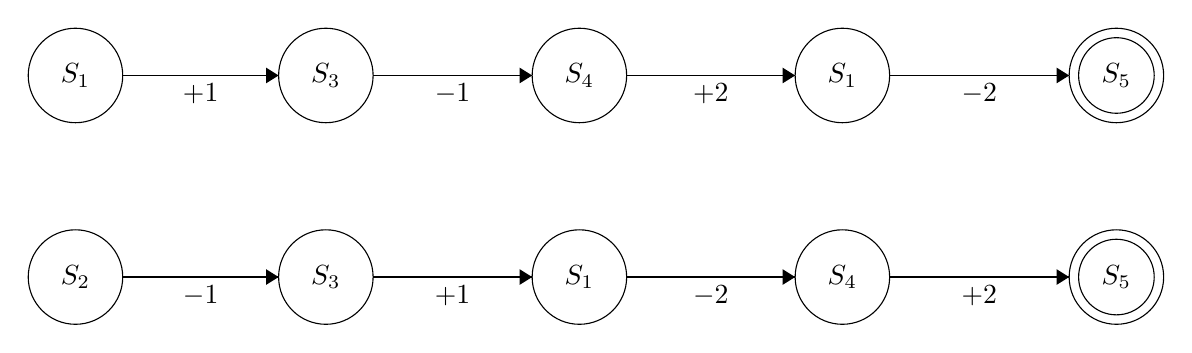
\begin{tikzpicture}[scale=0.2]
        \tikzstyle{every node}+=[inner sep=0pt]
        \draw [black] (7.6,-17.2) circle (3);
        \draw (7.6,-17.2) node {$S_1$};
        \draw [black] (23.5,-17.2) circle (3);
        \draw (23.5,-17.2) node {$S_3$};
        \draw [black] (39.6,-17.2) circle (3);
        \draw (39.6,-17.2) node {$S_4$};
        \draw [black] (56.3,-17.2) circle (3);
        \draw (56.3,-17.2) node {$S_1$};
        \draw [black] (73.7,-17.2) circle (3);
        \draw (73.7,-17.2) node {$S_5$};
        \draw [black] (73.7,-17.2) circle (2.4);
        \draw [black] (7.6,-30) circle (3);
        \draw (7.6,-30) node {$S_2$};
        \draw [black] (23.5,-30) circle (3);
        \draw (23.5,-30) node {$S_3$};
        \draw [black] (39.6,-30) circle (3);
        \draw (39.6,-30) node {$S_1$};
        \draw [black] (56.3,-30) circle (3);
        \draw (56.3,-30) node {$S_4$};
        \draw [black] (73.7,-30) circle (3);
        \draw (73.7,-30) node {$S_5$};
        \draw [black] (73.7,-30) circle (2.4);
        \draw [black] (10.6,-17.2) -- (20.5,-17.2);
        \fill [black] (20.5,-17.2) -- (19.7,-16.7) -- (19.7,-17.7);
        \draw (15.55,-17.7) node [below] {$+1$};
        \draw [black] (26.5,-17.2) -- (36.6,-17.2);
        \fill [black] (36.6,-17.2) -- (35.8,-16.7) -- (35.8,-17.7);
        \draw (31.55,-17.7) node [below] {$-1$};
        \draw [black] (42.6,-17.2) -- (53.3,-17.2);
        \fill [black] (53.3,-17.2) -- (52.5,-16.7) -- (52.5,-17.7);
        \draw (47.95,-17.7) node [below] {$+2$};
        \draw [black] (59.3,-17.2) -- (70.7,-17.2);
        \fill [black] (70.7,-17.2) -- (69.9,-16.7) -- (69.9,-17.7);
        \draw (65,-17.7) node [below] {$-2$};
        \draw [black] (10.6,-30) -- (20.5,-30);
        \fill [black] (20.5,-30) -- (19.7,-29.5) -- (19.7,-30.5);
        \draw (15.55,-30.5) node [below] {$-1$};
        \draw [black] (26.5,-30) -- (36.6,-30);
        \fill [black] (36.6,-30) -- (35.8,-29.5) -- (35.8,-30.5);
        \draw (31.55,-30.5) node [below] {$+1$};
        \draw [black] (42.6,-30) -- (53.3,-30);
        \fill [black] (53.3,-30) -- (52.5,-29.5) -- (52.5,-30.5);
        \draw (47.95,-30.5) node [below] {$-2$};
        \draw [black] (59.3,-30) -- (70.7,-30);
        \fill [black] (70.7,-30) -- (69.9,-29.5) -- (69.9,-30.5);
        \draw (65,-30.5) node [below] {$+2$};
    \end{tikzpicture}
\end{center}
We want to estimate the value-state function of $s_1$ using first visit
\begin{align*}
    \hat{V}^{\pi}_1(s_1) & = 1 - 1 + 2 - 2 = 0   \\
    \hat{V}^{\pi}_2(s_1) & = -2 + 2 = 0          \\
    \hat{V}^{\pi}(s_1)   & = \frac{0 + 0}{2} = 0
\end{align*}
Using every visit, we consider all the occurrences of $s_1$
\begin{align*}
    \hat{V}^{\pi}_{11}(s_1) & = 1 -1 +2 -2 = 0                            \\
    \hat{V}^{\pi}_{12}(s_1) & = -2                                        \\
    \hat{V}^{\pi}_{21}(s_1) & = -2 + 2 = 0                                \\
    \hat{V}^{\pi}(s_1)      & = \frac{(0) + (-2) + (0)}{3} = -\frac{2}{3}
\end{align*}
\newline
\par
\noindent
This two methods have different properties. First visit is unbiased. We know for the bias-variance tradeoff that, if we have low bias, we have high variance. So first visit is suited for problems with many many training samples. First visit will produce noisy estimation of the state-value function even with a decent amount of samples. This limits a lot the learning speed, because we need to calculate a lot of episodes. Every visit is consistent\footnotemark \footnotetext{An estimator is consistent if $\lim_{n \rightarrow \infty} \hat{x}_n = E[x]$. If we have infinite samples the estimator converges to the true value}. It has more bias and less variance compared to first visit. This can be explained by the fact that every visit considers some transitions of an episode multiple times, introducing bias. But, from the same number of episodes, it can extract more training samples reducing the variance.
From a computational point of view, it would be nice if we could calculate incrementally the empirical mean of the return. If we observe a new episode, we can update the mean without recalculating it from scratch.
\newpage
\begin{align*}
    \hat{\mu}_k & = \frac{1}{k} \sum_{j=1}^k x_j                                                                 \\
                & =\frac{1}{k} \bigg( x_k + \sum_{j=1}^{k-1} x_j \bigg)                                          \\
                & =\frac{1}{k} \bigg( x_k + (k-1) \hat{\mu}_{k-1} \bigg)                                         \\
                & =\hat{\mu}_{k-1} + \frac{1}{k}(x_k - \hat{\mu}_{k-1}) \numberthis \label{eqn-incremental_mean}
\end{align*}
In the MC case, using (\ref{eqn-incremental_mean}) we have
\begin{equation}
    V(s_t) \leftarrow V(s_t) + \frac{1}{N(s_t)}(v_t-V(s_t))
\end{equation}
where $N(s_t)$ is the number of times we have calculated the return for $s_t$.
This updates can be extended to non-stationary problems. In this cases is useful to forget old episodes.
\begin{equation}
    V(s_t) \leftarrow V(s_t) + \alpha(v_t-V(s_t))
\end{equation}
where $\alpha$ is a learning rate between zero and one. This has the result to weight more the new samples, because the weighting of $(v_t-V(s_t))$ doesn't converge to zero as in the case of $\frac{1}{N(s_t)}$, but remain constant.
\paragraph{Note - Characteristic recap}
\begin{itemize}
    \item Must work on episodic MDPs. To learn we use the entire episode
    \item Unlike dynamic programming, MC can evaluate at each episode only one choice at each state
    \item MC doesn't bootstrap. This term will be clear later
    \item Time required to estimate one state does not depend on the total number of states, but on the variance of the samples
\end{itemize}
\newpage
\subsubsection{Temporal difference learning (TD(0))}
Before explaining this new algorithm, it's worth recalling a very important learning rate property.
\begin{proposition}
    Let $X$ be a random variable in $[0, 1]$ with mean $\mu = E[X]$. Let $x_i \sim X$, $i=1,\dots,n$ be n i.i.d. realizations of $X$.
    Consider the following exponential estimator
    \begin{equation*}
        \mu_i = (1-\alpha_i) \mu_{i-1} + \alpha x_i
    \end{equation*}
    with $\mu_i=x_1$ and $\alpha_i$'s are learning rates.
    \newline
    If $\sum_i \alpha_i = \infty$ and $\sum_i \alpha_i^2 < \infty$, then $\hat{\mu}_n \overset{a.s.}{\rightarrow} \mu$. The estimator is consistent.
\end{proposition}
For example $\frac{1}{i}$ satisfies the above condition, and so produces a consistent estimator.
The very good thing about the estimator above is that, manipulating the learning rate, we can interpolate between the previous estimator value and the new sample. With $\alpha_i=0$ we are ignoring new sample and we keep unaltered our estimate. With $\alpha_i = 1$ we forget the previous estimate and we fully rely on the new sample. With $\alpha_i$ between zero and one we can decide how much we want to rely on the past or on the new sample. Keep in mind this concept, because it will be used for the temporal difference approach.
TD are a model-free methods which learn directly from the episodes experience. Differently from MC, it can use incomplete episodes to make guesses about the value functions. To do this, we have to estimate the return from a given state. For MC we have
\begin{equation*}
    V(s_t) \leftarrow V(s_t) + \alpha(\mathbf{v_t}-V(s_t))
\end{equation*}
For TD we simply substitute $v_t$ with $r_{t+1} + \gamma V(s_{t+1})$
\begin{equation*}
    V(s_t) \leftarrow V(s_t) + \alpha(\mathbf{r_{t+1} + \gamma V(s_{t+1})}-V(s_t))
\end{equation*}
Doing so, we can use partial rollout of an episodes, because we don't need the entire episode to estimate $r_t$. This practice is called bootstrapping. $r_{t+1} + \gamma V(s_{t+1})$ is called \textbf{TD target}. $\delta_t = r_{t+1} + \gamma V(s_{t+1}) - V(s_t)$ is called \textbf{TD error}.
\paragraph{Note - MC \& TD rewriting} We can observe that the MC and TD value function updates can be rewritten as we have seen in proposition 1.1.
For example for MC
\begin{align*}
    V(s_t) & \leftarrow V(s_t) + \alpha(v_t-V(s_t))        \\
           & \leftarrow V(s_t) + \alpha v_t- \alpha V(s_t) \\
           & \leftarrow (1-\alpha)V(s_t) + \alpha v_t
\end{align*}
As we have seen before, $\alpha$ balances the importance of new data versus old estimations.
\newline
\par
\noindent
We are sure that TD is a fairly biased, but consistent estimator. The high bias generates from bootstrapping, because at the beginning of the learning phase we rely on random, and so biased, estimates of the value-functions to estimate the return $v_t$.

\paragraph{Note - MC vs TD comparison}
\begin{itemize}
    \item \textbf{Episode termination} TD can learn online after every step. MC must wait until end of episode before return is known. TD can be use in continuing(non–terminating) environments. MC only works for episodic(terminating) environments
    \item \textbf{Bias-Variance} TD has low variance, some bias. MC has high variance, zero bias. TD is more used when the problem is Markovian. MC returns in non-Markovian problems.
\end{itemize}
\begin{center}
    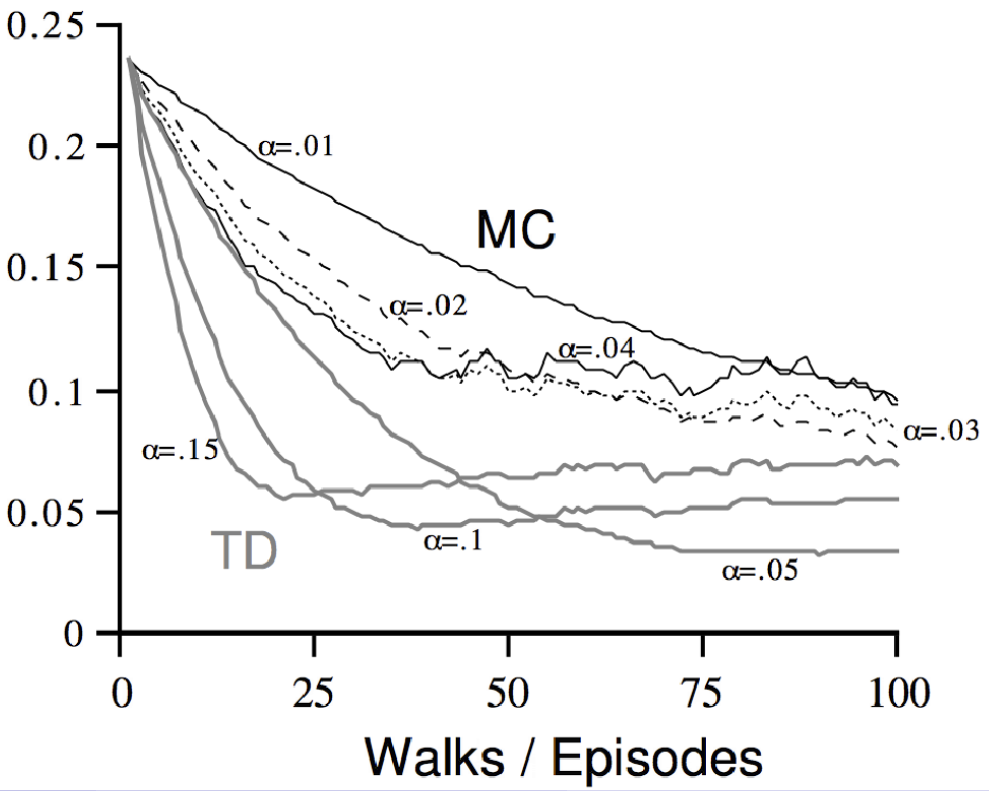
\includegraphics[width=120mm]{images/MCvsTD.PNG} \\
    \textit{RMS error averaged over states}
\end{center}
From the figure above we can observe some interesting properties. TD converges faster and has better results. The learning rate influences the convergence speed. Higher values will make the estimator converge faster, but the error will be higher. In TD this is due to the introduction of bias when we rely too much on new samples. When $\alpha$ is too large we are estimating the value function of a state, with another biased estimate of another state. This can clearly introduce some problems. MC suffers as well as TD with too high learning rates. The largest problem arises because of the large variance. We can see how with $\alpha=0.04$, MC becomes very noisy.

\subsubsection{\texorpdfstring{TD($\lambda$)}{TD(lambda)}}
We have seen how MC and TD have opposite characteristics in terms of bias-variance. It would be nice if we could choose which properties our algorithm should have. To do so, we can use TD($\lambda$). With the hyperparameter $\lambda \in [0,1]$, we can swing between TD with $\lambda=0$ and MC with $\lambda=1$.
\begin{center}
    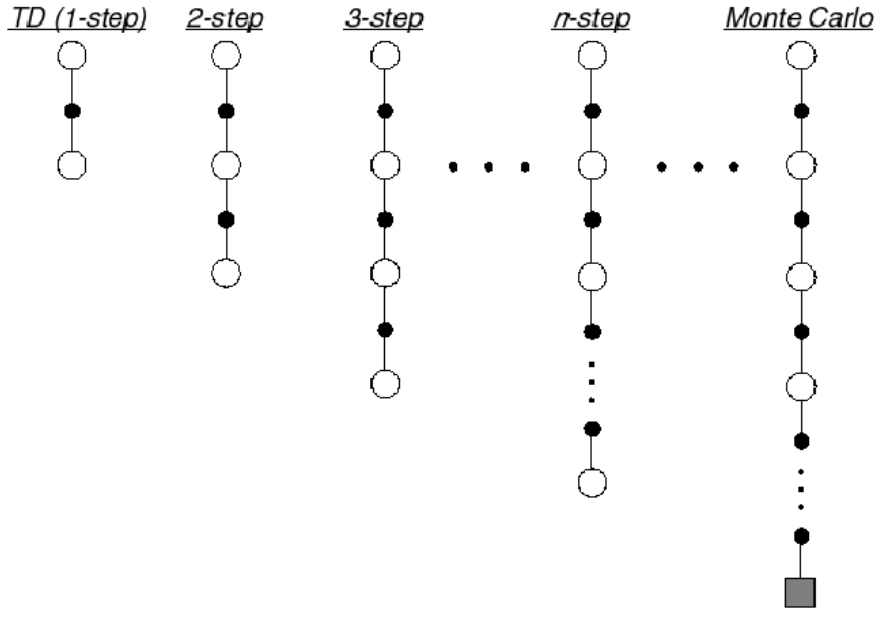
\includegraphics[width=100mm]{images/TD-N_step.PNG} \\
    \textit{Circles are states and dots are actions}
\end{center}
Before introducing formally the TD($\lambda$) equation  we have to define the n-step returns that we see in the figure above.
For $n=1,2,\dots,\infty$ the n-step return is
\begin{equation}
    v_t^{(n)} = r_{t+1} + \gamma r_{t+2} + \dots + \gamma^{n-1}r_{t+n} + \gamma^n V(s_{t+n})
\end{equation}
The n-step return is composed by n immediate rewards, plus the estimate of the state-value function in the upcoming state.
If we replace this estimator in the TD learning we get
\begin{equation*}
    V(s_t) \leftarrow V(s_t) + \alpha(v_t^{(n)}-V(s_t))
\end{equation*}
This isn't the TD($\lambda$) formula, but it gives us an intuition about the procedure. This approach has a problem. To calculate the n-step return we must perform n steps. We can't update our estimate of the state-value function at each step. To solve it, we can average the n-step returns after each step, to combine information from all steps.
In practice, we perform a weighted average called $\lambda$-return $v_t^{\lambda}$. Using weight $(1-\lambda)\lambda^{n-1}$,
\begin{equation}
    v_t^{\lambda} = (1-\lambda) \sum_{n=1}^{\infty} \lambda^{n-1} v_t^{(n)}
\end{equation}
We can use this new estimator in the TD learning formula
\begin{equation}
    V(s_t) \leftarrow V(s_t) + \alpha(v_t^{\lambda}-V(s_t))
\end{equation}

\begin{center}
    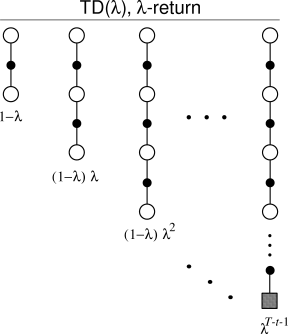
\includegraphics[width=60mm]{images/TDlambda.png}
\end{center}
This approach is called \textbf{Forward-view} TD($\lambda$). We can see that for $\lambda=0$, only the 1-step return have a weight different from zero. For $\lambda=1$, only the complete episode estimate have a weight different from zero. For values in between, we can give more importance to returns with fewer steps or give more weight to n-step returns with more steps. We can manage the bias-variance tradeoff by changing $\lambda$.
\paragraph{Note - Weights} As one can imagine, the weight formulation is very important. One of the most important property is that the weight must sum to 1. In our case, the sum of the weight is
\begin{align*}
    WeightSum & = (1-\lambda) \sum_{n=1}^{\infty} \lambda^{n-1}                                        \\
              & = \underbrace{\sum_{n=1}^{\infty} (1-\lambda) \lambda^n}_{\text{geometric series}} = 1 \\
\end{align*}
\begin{center}
    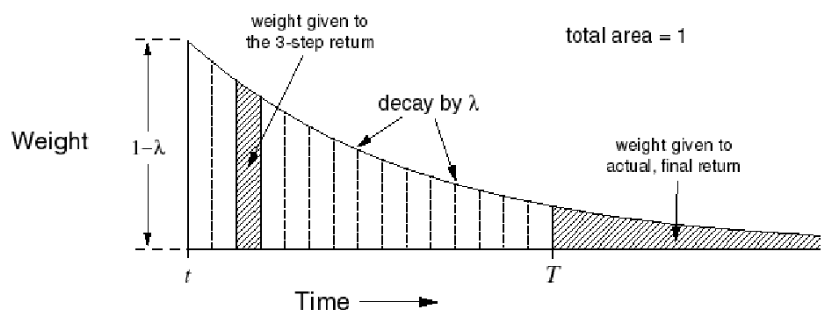
\includegraphics[width=120mm]{images/WeightDecay.PNG}
\end{center}
To recap, we want to estimate the state-value function of a state. Starting from the given state, at each step, we perform an action, stretching the trajectory length. Every step, we calculate the n-step return. To estimate the starting state value function, we average over the n-step returns obtained at each step, weighted with the hyperparameter $\lambda$. With this approach(forward-view), we still need to perform every step until we reach the complete episodes, because $v_t^{\lambda}$ still need the n-step return associated to the complete episode. To solve this problem we can use the so called \textbf{Backward-view} TD($\lambda$).
\par
\noindent
The forward-view provide us some the theory necessary to approach the problem. Backward-view gives us the mechanism. Our objective is to generate an algorithm capable of updating our estimate of the value function at each step. Our first step is to define the \textbf{eligibility traces}. The eligibility traces are used to solve the credit assignment problem, which consist in associating the merit of a given reward to a state. Given a trajectory, which states have influenced the most the reward? The eligibility traces are one of the many heuristic for solving the problem,
\begin{itemize}
    \item \textbf{Frequency heuristics} We assign credits to the most frequent state
    \item \textbf{Recency heuristics} We assign credit to the most recent states
    \item \textbf{Eligibility traces} We combine the frequency and recency heuristic\footnotemark \footnotetext{$+1(s=s_t)$ means that we add one only if the current state $s$ is equal to $s_t$}
          \begin{equation}
              e_{t+1}(s) = \underbrace{\gamma \lambda e_t(s)}_{\text{recency term}} + \underbrace{1(s=s_t)}_{\text{frequency term}}
          \end{equation}
          The eligibility trace is calculated in every state, and is update at each step.
          The frequency term makes the trace decay over time because $\gamma$(discount factor) and $\lambda$(TD hyperparameter) are less than one. The recency term adds one to the trace every time the state is visited.
\end{itemize}
\begin{center}
    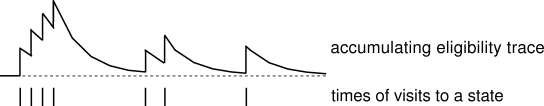
\includegraphics[width=120mm]{images/EligibilityTraces.png}
\end{center}
We have seen how the eligibility trace $e_t(s)$ measure the contribution of state s to the return. We can rewrite the state-value function including this term. For TD we had
\begin{align*}
    V(s_t) & \leftarrow V(s_t) + \alpha(r_{t+1} + \gamma V(s_{t+1})-V(s_t)) & \text{TD}                \\
           & \leftarrow V(s_t) + \alpha(\delta_t)                                                      \\
    V(s_t) & \leftarrow V(s_t) + \alpha(\delta_t e_t(s))                    & TD(\lambda)Backward-view
\end{align*}
TD($\lambda$) uses the eligibility traces to give more importance to the most recently or more frequently visited states. The states with high eligibility trace will rely more on newly seen data, by giving a boost to the learning rate.
\par
\noindent
Here we have the algorithm for backward-view TD($\lambda$)
\newline
\begin{algorithm}[H]
    \SetAlgoLined
    \SetKwInOut{Input}{Input}
    \SetKwInOut{Output}{Output}
    \SetKwInOut{Initialize}{Initialize}


    \Output{$V^{\pi}$}
    \Input{S, A, $\pi$, $\gamma$, $\lambda$}
    \Initialize{V(s) arbitrarily}
    \For{all episodes}{
        $e(s) \leftarrow 0$, $\forall s \in S$ \\
        $s \leftarrow$ starting state \\
        \Repeat{s is terminal}{
            $a \leftarrow$ action given by $\pi$ for $s$ \\
            Take action $a$, observe $r$, and next state $s'$ \\
            $\delta \leftarrow r + \gamma V(s') - V(s)$ \\
            $e(s) \leftarrow e(s) + 1$ \\
            \For{all $s \in S$}{
                $V(s) \leftarrow V(s) + \alpha \delta e(s)$ \\
                $e(s) \leftarrow \gamma \lambda e(s)$
            }
            $s \leftarrow s'$
        }
    }
    \caption{backward-view TD($\lambda$)}
\end{algorithm}
\par
\noindent
Using accumulating traces, frequently visited states can have eligibilities greater than one. This can be a problem for convergence. \textbf{Replacing traces}, instead of adding 1 when you visit a state, set that trace to 1.
\begin{equation}
    e_t(s) =
    \begin{cases}
        \gamma \lambda e_{t-1}(s), & \text{if }s \neq s_t \\
        1,                         & \text{if }s=s_t
    \end{cases}
\end{equation}
\begin{center}
    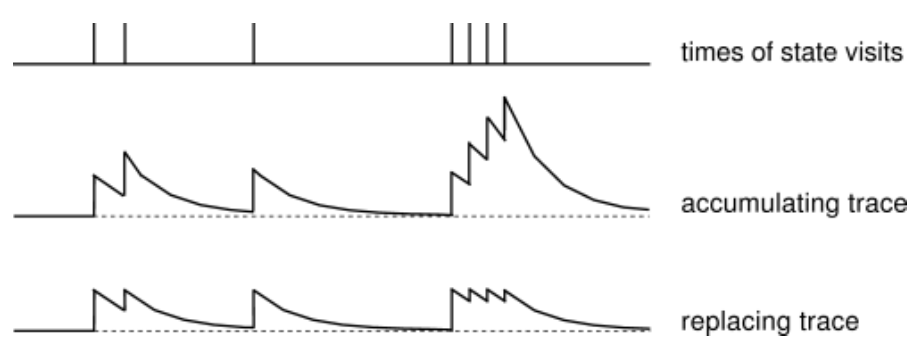
\includegraphics[width=120mm]{images/EligibilityTracesRepleacing.png}
\end{center}
\newpage

\subsection{Model-free control}
So far we have seen how to estimate the value function of a given policy. Now our objective is to find the policy $\pi^*$, that maximize the value function. We already done this in the previous chapter, under the assumption that we know the transition model of our problem. This is no longer true, so we need to modify our algorithms to accommodate this new situation.

\subsubsection{On-Policy-Monte-Carlo control}
This approach is based on policy iteration. As a reminder, policy iteration is divided in two steps, which are iterated until convergence. The first is policy evaluation. In this step we estimate the value function of our policy. Once we have an estimate, we can perform the second step, policy improvement. From the value function estimate, we can calculate the relative greedy policy, which we are sure is better then the previous policy. We iterate this two step until two consecutive policy evaluation are the same. The relative policy is the optimal one.
\par
\noindent
The policy evaluation step uses the transition model of the MDP. To solve this problem, we can use one of the model-free prediction algorithm we have seen in the previous section. For example we can use MC. We are done right? Not so fast. Now we can evaluate a policy model-free, but the policy improvement still needs the transition model, because it need to calculate the greedy policy.
\begin{equation*}
    \pi'(s) = \underset{a \in A}{argmax} \bigg\{ R(s,a) + \gamma \sum_{s' \in S} \mathbf{P(s'|s,a)} V(s') \bigg\}
\end{equation*}
We can do policy improvement model-free by using the action-value function
\begin{equation}
    \pi'(s) = \underset{a \in A}{argmax} \bigg\{ Q(s,a) \bigg\}
\end{equation}
In this way, we don't need anymore the transition model, because the greedy policy can be calculated by choosing the action that maximizes the action-value function in a state. In the policy evaluation step, we are no longer estimating $V$, but we have to calculate the action-value function $Q = Q^{\pi}$. We estimate the value of each state-action pair. Obviously the number of state-action pair are way more than the number of states, so we need to estimate more values than before. To compensate, we need to get more samples. Are we good? Not really unfortunately. Suppose to start our policy iteration with the random policy. We perform the policy evaluation step, and then we calculate the new greedy policy. Usually the greedy policy is deterministic. It means that in every state, we will always choose only one action. This is a problem, because to estimate $Q$ we need to explore all the state-action pair, but being deterministic we take always the same action in a given state. It happens that some state-action pairs will be never explored, and so we don't have a clue on the utility of the pair. The major consequence of this is that we can't use the greedy policy improvement as we have seen before, and furthermore we can't use deterministic policies using policy iteration to estimate $Q$. Here we can start to see one of the most important concept in RL. The \textbf{exploration vs exploitation dilemma}. This concept will be explained better in the next chapter, for now we say that when learning the value function of an MDP, we need to find the right balance between exploring the state-action pairs and exploiting the knowledge collected so far.
\par
\noindent
One of the easiest way to produce non-deterministic policies during the policy improvement step, is to use \textbf{$\mathbf{\epsilon}$ greedy exploration}. The policy will be calculated as follow
\begin{equation}
    \pi(s,a) =
    \begin{cases}
        \frac{\epsilon}{m}+1-\epsilon & \text{if }a^*=\underset{a \in A}{argmax} \{ Q(s,a) \} \\
        \frac{\epsilon}{m}            & \text{otherwise}
    \end{cases}
\end{equation}
Simplest idea for ensuring continual exploration. All the $m$ actions have non-zero probability of being chosen. The greedy action have a large probability of being chosen. $\epsilon$ manages the exploration-exploitation dilemma. Larger values of $\epsilon$ will generate policies which explore more, because it gives more probability to the non-greedy actions. The very good thing about $\epsilon$-greedy policy is its theoretical guarantees
\begin{theorem}[$\epsilon$-greedy policy improvement]
    For any $\epsilon$-greedy policy $\pi$, the $\epsilon$-greedy policy $\pi'$ with respect to $Q^{\pi}$ is an improvement
    \begin{align*}
        Q^{\pi}(s,\pi'(s)) & = \sum_{a \in A} \pi'(a|s) Q^{\pi}(s,a)                                                                                                                       \\
                           & = \frac{\epsilon}{m} \sum_{a \in A} \big( Q^{\pi}(s,a) \big) + (1-\epsilon) \max_{a \in A} Q^{\pi}(s,a)                                                       \\
                           & \geq \frac{\epsilon}{m} \sum_{a \in A} \big( Q^{\pi}(s,a) \big) + (1-\epsilon) \sum_{a \in A} \frac{\pi(a|s) - \frac{1}{\epsilon}}{1 - \epsilon} Q^{\pi}(s,a) \\
                           & = \sum_{a \in A} \pi(a|s) Q^{\pi}(s,a) = V^{\pi}(s)
    \end{align*}
    Therefore from policy improvement theorem, $V^{\pi'}(s) \geq V^{\pi}(s)$
\end{theorem}
\par
\noindent
This is great news, the $\epsilon$-greedy policy with respect to a policy is for sure better.
To recap we have,
\begin{itemize}
    \item \textbf{Policy evaluation} MC policy evaluation, $Q=Q^{\pi}$
    \item \textbf{Policy improvement} $\epsilon$-greedy policy improvement
\end{itemize}
As we have seen for DP policy iteration we don't need to calculate the true value function in the policy evaluation step, but we can stop when our approximation is close enough. In this case we have generalized model-free policy iteration
\begin{itemize}
    \item \textbf{Policy evaluation} MC policy evaluation, $Q \approx Q^{\pi}$
\end{itemize}
To completely define on-policy MC control, we still need some definitions.
\begin{definition}[GLIE]
    We say that an exploration strategy is Greedy in the Limit of Infinite Exploration(GLIE) if
    \begin{itemize}
        \item All state-action pair are explored infinitely many times
              \begin{equation*}
                  \lim_{k \rightarrow \infty} N_k(s,a) = \infty, \quad \forall(s,a)
              \end{equation*}
        \item The policy converges on a greedy policy
              \begin{equation*}
                  \lim_{k \rightarrow \infty} \pi_k(a|s) = \mathbf{1}(a = \underset{a' \in a}{argmax}\{ Q_k(s',a') \})
              \end{equation*}
    \end{itemize}
\end{definition}
\par\noindent
In GLIE MC control we have. Given sample $k^{th}$ episode using $\pi:\{ s_1,a_1,r_1,\dots,s_T \} \sim \pi$, for each state and action in the episode we have
\begin{align*}
    N(s_t,a_t)  & \leftarrow N(s_t,a_t) + 1                                      \\
    Q(s_t, a_T) & \leftarrow Q(s_t,a_t) + \frac{1}{N(s_T,a_t)}(v_t - Q(s_t,a_t))
\end{align*}
The policy improvement step based on the new action-value function will use
\begin{gather*}
    \epsilon \leftarrow \frac{1}{k} \\
    \pi \leftarrow \epsilon-greedy(Q)
\end{gather*}
\begin{theorem}[GLIE Monte-Carlo]
    GLIE Monte-Carlo converges to the optimal action-value function, $Q(s,a) \rightarrow Q^*(s,a)$
\end{theorem}
Now we have a way to find the optimal policy with a model-free approach.
\par\noindent
This method have many hyperparameters which are related to some time scales. We can recap their role and their relationship in order to make things clearer. There are three time scales,
\begin{itemize}
    \item \textbf{Behavioural} related to the discount factor $\gamma$. $\frac{1}{1-\gamma}$
    \item \textbf{Sampling} related to the learning rate $\alpha$ for the estimation of Q
    \item \textbf{Exploration} related to $\epsilon$, for the $\epsilon$-greedy strategy
\end{itemize}
To have good result during the learning phase, these three hyperparameters have to respect this relationship
\begin{equation*}
    1-\gamma \ll \alpha \ll \epsilon
\end{equation*}
As a starting point we can use $1-\gamma \approx \alpha \approx \epsilon$. Then we decrease $\epsilon$ faster than $\alpha$. We do so because if the learning rate is too small, while $\epsilon$ is still large, the exploration will not be counted. When updating our value function, $\alpha$ will weight more the old samples. This in practice, would ignore the newly explored states and actions.
Practically, given M trials we can set $\alpha \sim 1- \frac{m}{M}$ and $\epsilon \sim (1-\frac{m}{M})^2$. $\gamma$ should remains constant, because it is a property of the problem we are trying to solve, and not of the learning algorithm we are using. But in practice, $\gamma$ is initialized to low values, because the problem becomes easier. Then it is gradually moved towards its correct value. This approach is called curriculum learning.

\subsubsection{On-policy Temporal-Difference control}
As we did before, we can use temporal difference to solve the policy evaluation step. This approach have, as in the prediction case, a lot of advantages compared to MC. It has lower variance, it's online and it can work with incomplete sequences.
The most simple way to adapt the control problem using TD is by applying temporal difference to Q in the policy evaluation step. Then, we can use $\epsilon$-greedy policy improvement. These steps are done every time we take a new action.
\par \noindent
This on-policy control is called \textbf{SARSA}\footnotemark.\footnotetext{SARSA stands for: State Action Reward State Action} As in the MC case we need to evaluate the action-value function
\begin{equation*}
    Q(s,a) \leftarrow Q(s,a) + \alpha(r + \gamma Q(s',a') - Q(s,a))
\end{equation*}
At each time-step we perform
\begin{itemize}
    \item \textbf{Policy evaluation} SARSA, $Q \approx Q^{\pi}$
    \item \textbf{Policy improvement} $\epsilon$-greedy improvement
\end{itemize}

\begin{algorithm}[H]
    \SetAlgoLined
    \SetKwInOut{Input}{Input}
    \SetKwInOut{Output}{Output}
    \SetKwInOut{Initialize}{Initialize}
    \SetKwRepeat{Do}{do}{while}

    \Output{$Q^*$}
    \Input{S, A, $\pi_0$, $\gamma$, $\epsilon$}
    \Initialize{$Q(s,a)$ arbitrarily \\
        $\pi \leftarrow \pi_0$}

    \Do{convergence}{
        $s \leftarrow$ starting state \\
        $a \leftarrow$ action given by $\pi$ for $s$ \\
        \Repeat{$s$ is terminal}{
            Take action a, observe r, s'\\
            $a' \leftarrow$action given by $\pi$ for $s'$ \\
            $Q(s,a) \leftarrow Q(s,a) + \alpha[r + \gamma Q(s',a') - Q(s,a)]$ \\
            $s \leftarrow s'$ \\
            $a \leftarrow a'$ \\
            $\pi \leftarrow \epsilon$-greedy$(\pi)$
        }
    }
    \caption{SARSA On-Policy control}
\end{algorithm}
\par
\noindent
To ensure that the SARSA algorithm converges to the optimal solution, we have to check if some conditions are respected
\newpage
\begin{theorem}
    SARSA converges to the optimal action-value function, $Q(s,a) \rightarrow Q^*(s,a)$, under the following conditions
    \begin{itemize}
        \item GLIE exploration strategy(sequence of policies $\pi_t(s,a)$)
        \item Robbins-Monro sequence of step-sizes $\alpha_t$
              \begin{gather*}
                  \sum_{t=1}^{\infty} \frac{1}{\alpha_t} = \infty \\
                  \sum_{t=1}^{\infty} \frac{1}{\alpha_t^2} \leq \infty
              \end{gather*}
    \end{itemize}
\end{theorem}
We can see that for SARSA we are using TD(0), because we are bootstrapping after a single step. As we did before for the prediction problem, we can define a procedure which can swing across MC and TD with a parameter $\lambda$. This procedure is called SARSA($\lambda$)
\begin{itemize}
    \item \textbf{Forward view} update action–value $Q(s,a)$ to $\lambda$-return $v_t^{\lambda}$
    \item \textbf{Backward view} use eligibility traces for each state-action pairs.
          \begin{equation*}
              e_t(s,a) = \gamma \lambda e_{t-1}(s,a) + \mathbf{1}((s_t,a_t) = (s,a))
          \end{equation*}
\end{itemize}

\begin{algorithm}[H]
    \SetAlgoLined
    \SetKwInOut{Input}{Input}
    \SetKwInOut{Output}{Output}
    \SetKwInOut{Initialize}{Initialize}
    \SetKwRepeat{Do}{do}{while}

    \Output{$Q^*$}
    \Input{S, A, $\pi_0$, $\gamma$, $\lambda$, $\epsilon$}
    \Initialize{Q(s,a) arbitrarily \\
        $\pi \leftarrow \pi_0$}
    \Do{convergence}{
        $e(s,a) \leftarrow 0$, $\forall s,a$ \\
        $s \leftarrow$ starting state \\
        $a \leftarrow$ action given by $\pi$ for $s$ \\
        \Repeat{s is terminal}{
            Take action $a$, observe $r$, and next state $s'$ \\
            $a' \leftarrow$ action given by $\pi$ for $s'$ \\
            $\delta \leftarrow r + \gamma Q(s',a') - Q(s,a)$ \\
            $e(s,a) \leftarrow e(s,a) + 1$ \\
            \For{all $s,a$}{
                $Q(s,a) \leftarrow Q(s,a) + \alpha \delta e(s,a)$ \\
                $e(s,a) \leftarrow \gamma \lambda e(s,a)$
            }
            $s \leftarrow s'$ \\
            $a \leftarrow a'$ \\
            $\pi \leftarrow \epsilon$-greedy$(\pi)$
        }
    }
    \caption{Backward-view SARSA($\lambda$)}
\end{algorithm}
The preferred method for what we have seen before is the backward view.

\paragraph{Example - SARSA($\lambda$)} Imagine to have the gridworld in the figure below
\begin{center}
    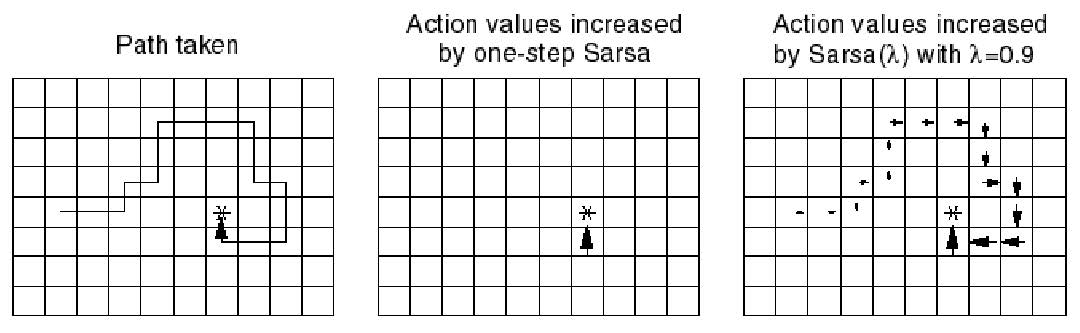
\includegraphics[width=120mm]{images/SARSA_Lambda_Comparison.jpg} \\
    \textit{From left to right: 1.Path taken 2.SARSA(0) 3.SARSA(0.9)}
\end{center}
Suppose to perform a complete episode of our MDP and we have estimated the action-value function with SARSA(0) and SARSA(0.9). The first corresponds to the TD approach. In fact, we update only the state-action pair right before the goal state, which is the only one returning a non-zero reward. All the other pairs are not updated because the goal return echoes only to the previous pair on the trajectory. On the other hand, With $\lambda=0.9$, the goal return is echoed through all the trajectory. We can also observe that the update decay over the trajectory, as we would expect.

\subsubsection{Off-Policy learning}
Off-policy methodologies try to estimate a policy that is different from the one generating the data. The estimated policy is called \textbf{target policy} $\pi(a|s)$, while the data generating one is called \textbf{behavior policy} $\Bar{\pi}(a|s)$. This could seem counter intuitive, but it can bring a lot of advantages to our learning phase. For example, splitting the two policy can give us an advantage when learning from observing humans or other agents, or reuse experience generated from old policies($\pi_1,\dots,\pi_{t-1}$). How can we estimate a policy from another one? We can use the concept of \textbf{importance sampling}. This method is used in general to estimate the expectation of a different distribution w.r.t. the distribution used to draw samples. Imagine to have a generic function $f(x)$. We sample $f(x)$ using a distribution $p$\footnotemark\footnotetext{Note that $f(x)$ is simply a generic function, for which we want to find the expected value. We want to estimate the expected value through sampling. To sample from the input space(x), we must use a probability distribution, in our case $p$}. To denote that the samples $x$ are drawn from $p$ we use $x \sim p$. The expected value of $f(x)$ can be written as $E_{x \sim p}[f(x)]$. Our objective is to find $E_{x \sim p}[f(x)]$ by sampling $x$ with another distribution $q$. We can manipulate the expected value to achieve this.
\begin{align*}
    E_{x \sim p}[f(x)] & = \int p(x)f(x) dx                                 \\
                       & = \int q(x) \bigg( \frac{p(x)}{q(x)}f(x) \bigg) dx \\
                       & =E_{x \sim q}\bigg[ \frac{p(x)}{q(x)}f(x) \bigg]
\end{align*}
We can see in the second line of the procedure, that we can consider as a new generic function $\frac{p(x)}{q(x)}f(x)$. Seeing that, we have an integral of a function, multiplied by a distribution $q$. This is by definition an expected value, with the samples drawn from $q$. In this way we can estimate the expected value of $f(x)$, by sampling from another distribution. The ratio $\frac{p(x)}{q(x)}$ is also called \textbf{importance weight} $W(x)$. We can guess that this ratio weights the importance of the given sample. When $p$ gives a big importance to a region, and $q$ doesn't, we must amplify the sample, if we have taken it from $q$. In $p$ we sample frequently a given region. In $q$ we sample rarely, but when applying importance sampling every sample from that region have a large weight to compensate. In fact when $p(x)$ is large and $q(x)$ is small $W(x)$ becomes bigger. Importance sampling is like doing a weighted average, where the samples are weighted according to their importance.

In our RL problem, we can use it at our advantage. If we consider as our generic function the return $v_t$, and as sampling distributions the target policy $\pi$ and behavior policy $\Bar{\pi}$, we can apply importance sampling\footnotemark.\footnotetext{$f(x) \rightarrow v_t$, $p(x) \rightarrow \pi$, $q(x) \rightarrow \Bar{\pi}$} Assume to use a MC approach, so we estimate the return with the whole trajectory. Using $\Bar{\pi}$, we obtain at the end of an episode the return $v_t$, Then, we weight using importance sampling the return obtained obtaining $v_t^{\mu}$.
\begin{equation}
    v_t^{\mu} = \frac{\pi(a_t|s_t) \pi(a_{t+1}|s_{t+1})}{\Bar{\pi}(a_t|s_t) \Bar{\pi}(a_{t+1}|s_{t+1})} \dots \frac{\pi(a_T|s_T)}{\Bar{\pi}(a_T|s_T)} v_t
\end{equation}
Once we obtained the re-weighted return, we can update the action-value function using $v_t^{\mu}$
\begin{equation}
    Q(s_t,a_t) \leftarrow Q(s_t,a_t) + \alpha(v_t^{\mu} - Q(s_t,a_t))
\end{equation}
The behavior policy must be chosen very wisely. It has to be very close to the target policy, otherwise the estimation variance grows dramatically. In particular we must use a $\Bar{\pi}$ that is zero where $\pi$ is zero.

We can also use importance sampling with SARSA. In this case we get much better results compared to MC.
We use TD targets generated from $\Bar{\pi}$ to evaluate $\pi$. In practice with importance sampling, we weight the TD target $r+ \gamma Q(s',a')$ according to the similarity between the two policies. As we have seen before, with SARSA we perform a step and then we evaluate the action-value function. Doing so, we only need a single importance sampling correction at each step
\begin{equation}
    Q(s_t,a_t) \leftarrow Q(s_t,a_t) + \alpha \bigg( r_{t+1}+ \gamma \frac{\pi(a_{t+1}|s_{t+1})}{\Bar{\pi}(a_{t+1}|s_{t+1})} Q(s_{t+1},a_{t+1}) - Q(s_t,a_t) \bigg)
\end{equation}
With SARSA we have much lower variance than Monte–Carlo importance sampling and policies only need to be similar over a single step.
\newpage

\paragraph{Off–Policy Control with Q–learning}
Q-learning is the most used RL algorithm. It's very similar to SARSA,
\begin{equation}
    Q(s,a) \leftarrow Q(s,a) + \alpha (r + \gamma \max_{a' \in A}\{ Q(s',a') \} - Q(s,a))
\end{equation}
We can see how the only difference is the usage of the max operator in the TD target. This little difference makes a lot of difference. First of all, the algorithm becomes off-policy, because the next action $a'$ in the TD target is decided using the greedy policy in the current state, and not using the policy $\pi$. Most importantly, we can demonstrate that Q-learning converges to the optimal $Q^*$ even when the GLIE condition is not respected. This means that we don't have to stop exploring in order to converge to the optimal solution. The algorithm is so solid that, even if we use always the random policy the algorithm will converge to the optimal solution. As SARSA can be seen as the model-free version of policy iteration, Q-learning can be seen as the model-free version of value iteration. In fact, we can see how Q-learning uses the optimal Bellman operator over the single step. Note that, to choose the actual action $a$ in a given state we use the policy $\pi$ derived from the $\epsilon$-greedy improvement. To estimate the next action $a'$ we use the greedy policy of $\pi$.

\begin{algorithm}[H]
    \SetAlgoLined
    \SetKwInOut{Input}{Input}
    \SetKwInOut{Output}{Output}
    \SetKwInOut{Initialize}{Initialize}
    \SetKwRepeat{Do}{do}{while}

    \Output{$Q^*$}
    \Input{S, A, $\pi_0$, $\gamma$, $\epsilon$}
    \Initialize{Q(s,a) arbitrarily \\
        $\pi \leftarrow \pi_0$}
    \Do{convergence}{
        $s \leftarrow$ starting state \\
        \Repeat{s is terminal}{
            $a \leftarrow$ action given by $\pi$ for $s$ \\
            Take action $a$, observe $r$, and next state $s'$ \\
            $Q(s,a) \leftarrow Q(s,a) + \alpha(r + \gamma \max_{a' \in A}\{ Q(s',a') \} - Q(s,a))$ \\

            $s \leftarrow s'$ \\
            $\pi \leftarrow \epsilon$-greedy$(\pi)$
        }
    }
    \caption{Q-learning}
\end{algorithm}

\newpage
\end{document}
